\documentclass{article}
\usepackage[utf8]{inputenc}
\usepackage{graphicx}
\usepackage{subcaption}
\usepackage{amsmath}
\usepackage[nottoc]{tocbibind}
\usepackage{url}

\title{MATH DATA 195M Final Project: Supertasks}
\author{Vatsav Sethupathi}
\date{14th April 2020}

\begin{document}

\maketitle

\section{Introduction}
Consider the following thought experiment where you are given a cake and a knife which is meant to cut the cake. You are told to keep cutting the cake in half and stack the smaller half pieces on top of each other. This process slowly creates a pattern. We start to notice that every successive cut yields a shape which has the original volume of the cake that we began with, but the surface area for the same keeps increasing. If we keep cutting this cake for an infinite amount of time, we are theoretically left with a cake that has a pre-determined, fixed volume, but an infinite surface area. In essence, we have managed to create a \textsl{Supersolid}.

\section{Supersolids and Gabriel's Horn}
As highlighted by the thought experiment above, a supersolid is a geometric figure which has an infinite surface area, but a finite volume. An example of a supersolid would be the cake that we managed to create above. This cake is known as \textsl{Gabriel’s cake}, and is based on another supersolid called \textsl{Gabriel’s Horn}. This name refers to the Abrahamic tradition that identifies the Archangel Gabriel as the angel who blows the horn to announce Judgement day, thereby associating the divine, or infinite, with the finite.\cite{Wikipedia}

\subsection{A Mathematical representation of Gabriel's Horn}
In mathematical terms, \textsl{Gabriel’s Horn} can be represented using the graph of $\frac{1}{x}$. Using improper integrals, it is possible to find the area and the volume of the shape formed by this graph when it is rotated along the line y = 0. \cite{Wolfram}

\begin{figure}[h]
    \centering
    \begin{subfigure}[b]{0.4\linewidth}
      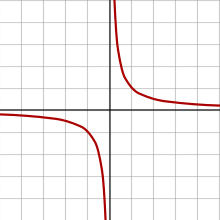
\includegraphics[width=\linewidth]{Graph 1.png}
      \caption{2D Graph of $\frac{1}{x}$}
    \end{subfigure}
    \hspace{4mm}
    \begin{subfigure}[b]{0.4\linewidth}
      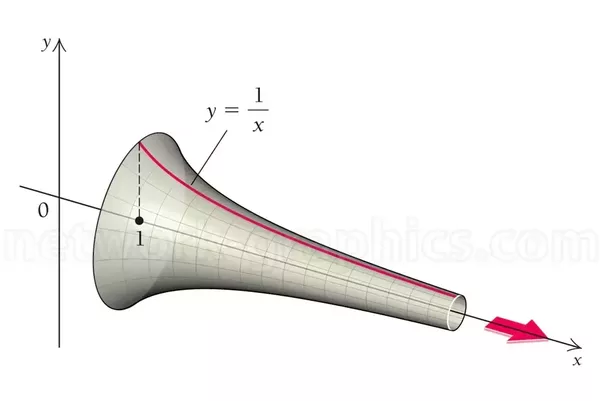
\includegraphics[width=\linewidth]{Graph 2.png}
      \caption{Graph of $\frac{1}{x}$ rotated along x=0}
      \begin{minipage}{.1cm}
      \vfill
      \end{minipage}
    \end{subfigure}
    \caption{The graphs of $\frac{1}{x}$ in 2 and 3 dimensions}
    \label{fig:my_label}
\end{figure}

\begin{equation}
  \begin{split}
    A & = \lim_{a\to\infty} 2\pi \int_{1}^{a} \frac{1}{x} \sqrt{1 + \left( -\frac{1}{x^2} \right)^2} dx > \lim_{a\to\infty} 2\pi \int_{1}^{a} \frac{dx}{x} \\
    \vspace{3mm}
    & = \lim_{a\to\infty} 2\pi ln(a)\\
    & = \infty.
  \end{split}
\end{equation}

\begin{equation}
    \begin{split}
        V & = \lim_{a\to\infty} \pi \int_{i}^{a} \left( \frac{1}{x} \right) ^2 dx \\
        & = \lim_{a\to\infty} \pi \left(1 - \frac{1}{a} \right) \\
        & = \pi \cdot \lim_{a\to\infty} \left(1 - \frac{1}{a} \right) \\
        & = \pi.
    \end{split}
\end{equation}

\subsection{Creating Gabriel's Horn}
As we can see, although the volume of the shape is finite (the volume converges to $\pi$ to be specific), the surface area of the graph diverges, that is, it tends to $\infty$. As a result, building such a solid in the real world is met with several inherent difficulties. Take for example, \textsl{Gabriel’s Cake}: no matter how many cuts we make, it will always have to be followed by another one, thereby requiring an infinite amount of time to complete its construction. This paradox, however, could be addressed with the introduction of a concept called the \textsl{Supertask}. 

\section{What is a Supertask?}
Consider the same thought experiment as before, but with a twist. This time, we are told to complete the construction of \textsl{Gabriel’s cake} in 2 mins. Now, instead of performing each cut at a constant rate, we decide to do so at an accelerated pace. We can make the first cut and then wait 1 minute to make the next one. Then, after this slice, we wait 30 seconds to make the next one, then 15 seconds to cut again, and so on. Since we can keep dividing the time required in half forever, there will always be another step. No matter how many steps we complete, there will always be an infinite amount of steps ahead. However, once the allotted amount of time is elapsed, each of these steps would have been completed. \textbf{This concept of completing an infinite number of tasks in a finite amount of time is what is referred to as a Supertask.} \cite{sep-spacetime-supertasks}


\section{Zeno's Dichotomy}
One of the most celebrated examples of a supertasks is \textsl{Zeno’s Dichotomy}, according to which a runner (in this case, the Greek Hero Achilles) can never complete a race since he must first run to the half way point, and then to the half way point of the remainder and so on indefinitely. Since there is always another half-way point to reach, there is no ‘final’ destination after which Achilles’ next stop is the finish line. Despite the unending nature of this task, Achilles manages to complete the race. \cite{Earman-Norton} 

\vspace{3mm}

The mathematician Max Black, however, was unconvinced. Like most modern skeptics of the standard resolution, he accepted that the total distance traversed $\frac{1}{2} + \frac{1}{4} + \frac{1}{8} + $... $$\left( D = \sum_{n=1}^{\infty} \frac{1}{2^{n}} \right)$$ approaches the finite value of unity in some suitable sense of the limit. The difficulty he identified lay deeper. He reasoned that it is logically impossible to complete an infinite number of journeys in a finite time, no matter how much faster or easier each successive journey becomes. \cite{Earman-Norton}

\section{A Possible Solution}
% Must add citation in line 3
John Wisdom agreed in the main with Black but added his own alternative resolution which appealed to the idea that points of physical space and time have a finite extension.\cite{Earman-Norton} Although the problem itself is logically impossible to complete, real world assumptions and theories help debunk the experiment and provide an explanation to the seemingly impossible completion of the race. In our real world understanding of science, there exists a certain distance which cannot be meaningfully divided any further. The only possible next position after reaching this distance is the finish line. This distance is known as the \textsl{Planck Length} and is mathematically equivalent to one hundred quintillionths of a proton’s diameter $\left( 1.61623 \cdot 10^{-35} m \right)$. However, taking to the real world could just be an excuse to avoid the problem itself. As John Earman complains, “It seems unattractive to make the truth of mathematical statements depend on the contingencies of space and time.” Therefore, we can think of supertasks not as a method to try and explain the structure of space and time, but much rather a way to demonstrate humans' incredible ability to confuse themselves.

\section{Paradoxes in Supertasks}
Consider the same example of Zeno’s Dichotomy, except in this case, the runner alternatively holds up a red or a blue flag at every step. Which color would he be holding up at the end of the race? Any answer seems wrong in this case as it would seem to suggest that the largest number (if it exists) is either odd or even. Take the case of another famous example of supertasks, namely Thomson’s lamp. This task, devised by James F. Thomson, consists of a lamp that can turned on and off as fast as we want. Imagine if we turn this lamp on and off Zenomially, i.e. in an accelerated fashion, like a supertask. At the end of the supertask, would this lamp be on or off? Again, any answer that we would give will sound absurd because every time the lamp is turned on there is a later moment where it is also turned off and vice versa. This introduces a paradox in our consideration of the supertask. A paradox that, according to Thomson, suggests that this supertask associated with the lamp is impossible! \cite{sep-spacetime-supertasks}.

\section{The Bouncing Ball : A Solution to the Paradox}
One of the best solutions to this seemingly impossible supertask is provided by Paul Benaceraff. Is Thomson's lamp on or off at the completion of the supertask? Benaceraff states that the answer to this question is unknown. This is primarily due to the fact that the question itself is incomplete!\cite{Benacerraf} Although supertasks are finite in duration, they have an endless amount of steps and ask us about the end. Thomson's lamp asks a question that is analogous to asking whether a lamp in a locked room is on or off. We have no way of knowing! In order to solve these questions, Benaceraff states that these questions need to be reworded, or coupled with more assumptions.\cite{Benacerraf}

\vspace{3mm}

Assume that Thomson's lamp is connected to a circuit that is operated using a Bouncing Ball. This ball completes the circuit each time it bounces and switches the lamp on or off. Assuming ideal physical conditions, lets say that the ball bounces half as high as it did in its previous bounce every time. This sequence of bounces will turn the lamp on and off an infinite number of times in a finite period of time. These assumptions allow us to finally propose a solution to Thomson's lamp. Although the lamp has no penultimate step, it does have a final resting position. This final state concludes that the ball will lie on the ground and the circuit will be complete, thereby leaving the lamp on!\cite{Earman-Norton} Using these additional assumptions, Benaceraff was finally able to put the debate to rest by providing a solution that is somewhat acceptable while operating under the conditions of ideal physics.

\section{Conclusion}
Over the centuries, paradoxes of infinity have played an honorable role in pointing to fundamental questions in logic, mathematics, and the physics of motion. However, we are not so naive as to think that we have had the last word on supertasks \cite{Earman-Norton}. The bigger question now becomes, ‘So what? Who cares?’ We will never build a lamp that turns on and off arbitrarily fast, and neither will we make a cake that has an infinite surface area. This is where we are introduced to the beauty of supertasks. They are nothing but philosophically interesting puzzles, or entertaining riddles. They are the human race’s demonstration that we can ask more questions than we can answer. This unending thirst to solving problems and creating more impossible ones is what has fostered the growth of human society and will continue to do so in the years to come. Ironically, this in itself might turn out to be a supertask of its own.

\bibliography{info}
\bibliographystyle{plain}

\vspace{10mm}

Word count = 1490 words

\end{document}
